\section{Problem and Data Description}
\label{sec:data}
\subsection{Problem Formulation and Research Questions}
Low-resolution product images provide a controlled setting for studying how model
structure affects classification. Fashion-MNIST includes visually similar garments,
so success requires distinguishing shape and texture rather than exploiting a class
frequency. We compare five implementations on a fixed partition and evaluation protocol.

Each input is a grayscale image \(X_i\in\mathbb{R}^{1\times28\times28}\) with one label
\(y_i\in\{0,\ldots,9\}\). A classifier produces ten raw scores:
\[
 f_\theta(X_i)=z_i\in\mathbb{R}^{10},\qquad
 \widehat y_i=\arg\max_{k\in\{0,\ldots,9\}} z_{i,k}.
\]
The objective is mean multiclass cross-entropy; probabilities are recorded for
interpretation, not supplied to the loss. The prediction unit is one image.
The comparison addresses four questions:
\begin{enumerate}
\item How do Linear, MLP, CNN, GRU and Transformer configurations compare in held-out
test accuracy and macro-F1?
\item How do flattened, spatial, row-sequence and patch-sequence representations relate
to their strengths and class-specific errors?
\item What trade-offs arise among predictive quality, parameter count, training cost
and measured CPU inference cost?
\item How much do results vary across training seeds 69420, 67 and 69?
\end{enumerate}
The results describe the tested configurations. Parameter count, optimization policy
and regularization also vary, so differences cannot be attributed solely to architecture.

\subsection{Dataset Description and Provenance}
Fashion-MNIST is the Zalando Research benchmark introduced by Xiao et al.\citep{fashion}
Its official sources contain 60,000 training and 10,000 test images, each an 8-bit
\(28\times28\) grayscale array, with ten labels and 7,000 examples per class across
both sources. The official repository publishes the dataset under the MIT
license.\citep{fashionlicense} Our loaders use
\texttt{torchvision.datasets.FashionMNIST} and the original IDX resources, without
changing the label mapping. CSV exports are not used by the training pipeline.

The original authors derive the benchmark from front-view catalog thumbnails.
Their conversion includes background-border trimming, subsampling, sharpening,
canvas centering, intensity inversion and grayscale conversion.\citep{fashion}
These are dataset-construction operations. The group starts from the distributed
IDX images and applies the separate transformations in Section~\ref{sec:preprocess}.
This distinguishes the dataset authors' processing from our code.

Raw IDX images have a 16-byte header and label files an 8-byte header.
Table~\ref{tab:inventory} records byte counts of the cached canonical resources used
for report verification. Each gzip resource was checked against the MD5 value in
torchvision's resource list, and decompression matched the IDX file byte-for-byte.
These are actual gzip sizes, rather than a generic archive-viewer size column.
\begin{table}[H]\centering\small
\caption{Verified canonical Fashion-MNIST resources in the local cache.}
\label{tab:inventory}
\begin{tabular}{lrr}
\toprule
Canonical resource & IDX bytes & Gzip bytes \\
\midrule
train-images images & 47,040,016 & 26,421,880 \\
train-labels labels & 60,008 & 29,515 \\
t10k-images images & 7,840,016 & 4,422,102 \\
t10k-labels labels & 10,008 & 5,148 \\
Total & 54,950,048 & 30,878,645 \\
\bottomrule
\end{tabular}

\end{table}
The four uncompressed IDX files occupy 54,950,048 bytes. This inventory describes
the cached resources; it does not assert an undocumented Kaggle acquisition session.

Limitations include small grayscale inputs, catalog-style backgrounds and overlapping
visual definitions among tops, shirts, pullovers and coats. Balanced label counts
do not remove content bias, annotation ambiguity or the domain gap from real photographs.

\subsection{Exploratory Data Analysis}
The saved stratified partition has exactly 5,000 training and 1,000 validation
examples per class; each official-test class also has 1,000 examples.
Table~\ref{tab:counts} was checked against the saved indices and raw labels.
The largest-to-smallest count ratio is 1.0 in each partition, so label imbalance
does not motivate resampling or class weighting here.
\begin{table}[H]\centering\small
\caption{Class support in the fixed seed-36 split.}
\label{tab:counts}
\begin{tabular}{rlrrr}
\toprule
ID & Class & Train & Validation & Test \\
\midrule
0 & T-shirt/top & 5000 & 1000 & 1000 \\
1 & Trouser & 5000 & 1000 & 1000 \\
2 & Pullover & 5000 & 1000 & 1000 \\
3 & Dress & 5000 & 1000 & 1000 \\
4 & Coat & 5000 & 1000 & 1000 \\
5 & Sandal & 5000 & 1000 & 1000 \\
6 & Shirt & 5000 & 1000 & 1000 \\
7 & Sneaker & 5000 & 1000 & 1000 \\
8 & Bag & 5000 & 1000 & 1000 \\
9 & Ankle boot & 5000 & 1000 & 1000 \\
\bottomrule
\end{tabular}

\end{table}

Figure~\ref{fig:representatives} shows the first four saved training indices of
each category. These are unaugmented training images, not examples chosen using
test performance. Their variation and shared upper-body silhouettes suggest
plausible sources of confusion.
\begin{figure}[H]\centering
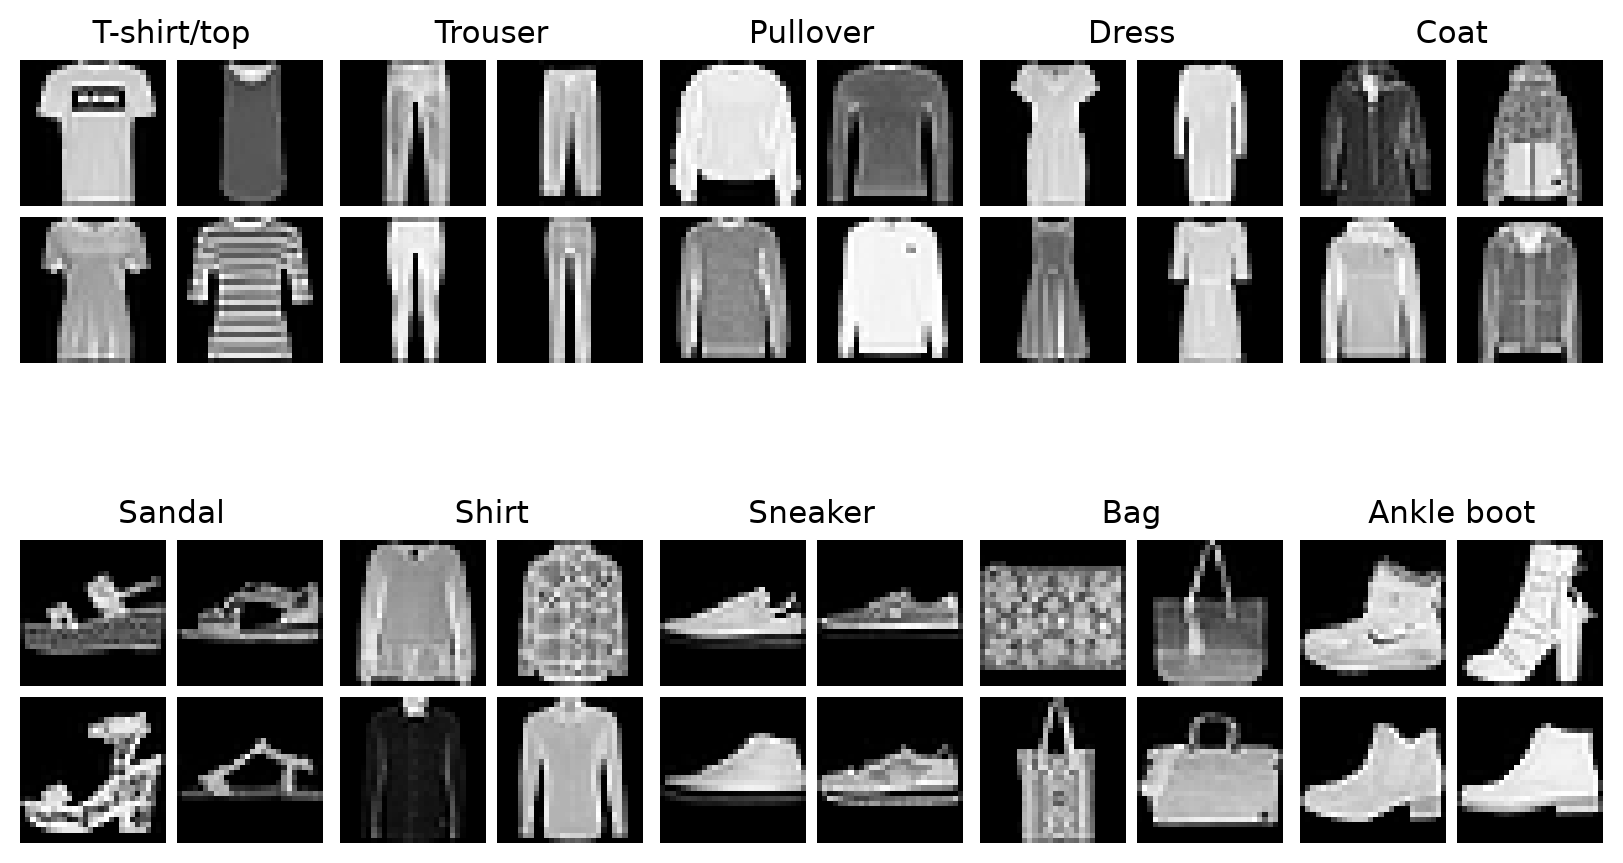
\includegraphics[width=\linewidth]{figures/training_examples.png}
\caption{Forty representative training images: four examples per class panel.
Selection IDs are retained in \texttt{evidence/eda\_selection.json}.}
\label{fig:representatives}
\end{figure}
Visual similarity alone does not establish prediction confidence. Actual probabilities
and confusion frequencies are examined in Sections~\ref{sec:confusion}
and~\ref{sec:qualitative}. No manual relabeling, perceptual duplicate removal or
custom outlier filtering was performed.

\subsection{Data Splitting and Leakage Prevention}
The official training source is stratified into 50,000 training and 10,000 validation
images with split seed 36. The official 10,000-example test source remains separate.
The persisted manifest is \path{configs/a1/splits/fashion_mnist_split.json};
ordinary loader construction reads it instead of resampling a new split.

The validator checks index ranges, duplicates, full source coverage and disjoint
training/validation membership. Test indices use a different source namespace even
when their integer values coincide with training indices. Normalization is fitted
on unaugmented training indices only. Validation selects checkpoints; final test
scores do not select a checkpoint or the best seed.

The short excerpt below uses the implementation's actual manifest fields:
\begin{lstlisting}[style=pythoncode]
train_indices = manifest.train_indices
val_indices = manifest.validation_indices
test_indices = manifest.test_indices
\end{lstlisting}
These controls prevent index overlap and normalization leakage. They do not establish
that visually duplicated product images have been removed across partitions;
no perceptual-duplicate audit is claimed.

\subsection{Preprocessing, Augmentation and Example Batch}
\label{sec:preprocess}
All five main configurations use the same training-only random crop:
\(28\times28\) output after two pixels of zero-valued constant padding per side.
No horizontal flip is enabled. Tensor conversion scales uint8 pixels to \([0,1]\),
then applies the training-derived statistics:
\[
 \mu=0.28585961086061534,\qquad
 \sigma=0.352790375749525,\qquad x'=(x-\mu)/\sigma.
\]
Validation and test apply tensor conversion and this normalization without random
augmentation. Their values do not contribute to fitting the statistics.

Every reported main run has configured batch size 64 and retains the last incomplete
batch. The shared contract is float32 images \([B,1,28,28]\), int64 labels \([B]\),
and \(B\) stable sample IDs. For instance,
\texttt{fashion\_mnist:official\_test:0} identifies an original test image, not a
batch-relative position.

Figure~\ref{fig:batch} shows six entries of a 64-example batch regenerated for the
report from saved training indices, using crop RNG seed 69420 and the same transform
definition. This is a post-hoc data illustration, not a logged training-epoch batch.
Its actual shape is \([64,1,28,28]\), dtype float32, and observed normalized range
approximately \([-0.8103,2.0243]\). The display maps that fixed range to grayscale.
\begin{figure}[H]\centering
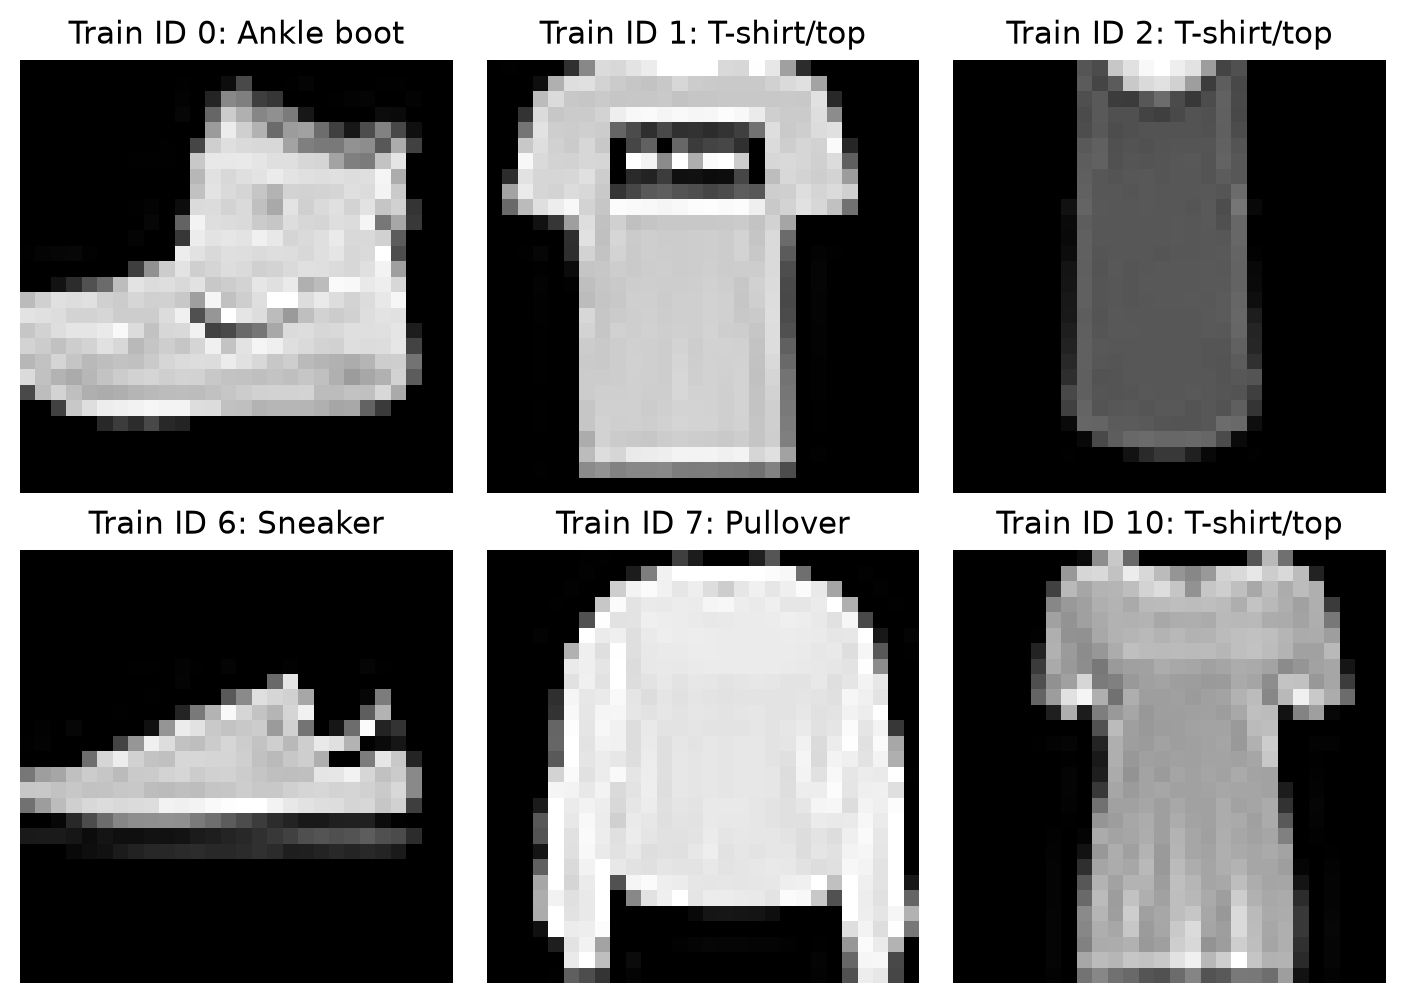
\includegraphics[width=.90\linewidth]{figures/preprocessed_batch.png}
\caption{Post-hoc example training batch after crop and normalization. Six of 64
images are shown; IDs/statistics are saved in \texttt{evidence/example\_batch.json}.}
\label{fig:batch}
\end{figure}
\FloatBarrier
